\documentclass{beamer}
\usepackage[utf8]{inputenc}

\usetheme{Madrid}
\usecolortheme{default}
\usepackage{amsmath,amssymb,amsfonts,amsthm}
\usepackage{txfonts}
\usepackage{tkz-euclide}
\usepackage{listings}
\usepackage{adjustbox}
\usepackage{array}
\usepackage{tabularx}
\usepackage{gvv}
\usepackage{lmodern}
\usepackage{circuitikz}
\usepackage{tikz}
\usepackage{graphicx}

\setbeamertemplate{page number in head/foot}[totalframumber]

\usepackage{tcolorbox}
\tcbuselibrary{minted,breakable,xparse,skins}

\definecolor{bg}{gray}{0.95}
\lstset{
    language=C,
    basicstyle=\ttfamily\small,
    keywordstyle=\color{blue},
    stringstyle=\color{orange},
    commentstyle=\color{green!60!black},
    numbers=left,
    numberstyle=\tiny\color{gray},
    breaklines=true,
    showstringspaces=false,
}

%------------------------------------------------------------
\title{1.4.21}
\date{August 28,2025}
\author{EE25BTECH11006 - ADUDOTLA SRIVIDYA}

\begin{document}

\frame{\titlepage}

\begin{frame}{Question}
Find the coordinates of the point which divides the line segment joining $\vec{A}(2,3)$ and $\vec{B}(6,-3)$ in the ratio $2:3$ \textbf{internally and externally}.
\end{frame}

\begin{frame}{Formula}
The section formula for a point $\vec{P}$ dividing $\vec{A}$ and $\vec{B}$ in the ratio $m:n$ is:
\begin{align}
\vec{P} = \frac{m\vec{B}+n\vec{A}}{m+n} \quad &\text{(Internal Division)} \\
\vec{P} = \frac{m\vec{B}-n\vec{A}}{m-n} \quad &\text{(External Division)}
\end{align}
\end{frame}

\begin{frame}{Internal Division}
Here, $m=2$, $n=3$, $\vec{A}=\begin{bmatrix}2\\3\end{bmatrix}$, $\vec{B}=\begin{bmatrix}6\\-3\end{bmatrix}$.
\begin{align}
\vec{P}_{int} &= \frac{2\begin{bmatrix}6\\-3\end{bmatrix}+3\begin{bmatrix}2\\3\end{bmatrix}}{2+3} \\
&= \frac{1}{5}\begin{bmatrix}12+6 \\ -6+9\end{bmatrix} = \frac{1}{5}\begin{bmatrix}18\\3\end{bmatrix} \\
&= \begin{bmatrix} \tfrac{18}{5} \\ \tfrac{3}{5} \end{bmatrix} = \brak{3.6, 0.6}
\end{align}
\end{frame}

\begin{frame}{External Division}
\begin{align}
\vec{P}_{ext} &= \frac{2\begin{bmatrix}6\\-3\end{bmatrix}-3\begin{bmatrix}2\\3\end{bmatrix}}{2-3} \\
&= \frac{1}{-1}\begin{bmatrix}12-6 \\ -6-9\end{bmatrix} \\
&= \begin{bmatrix}-6 \\ 15\end{bmatrix}
\end{align}
So the external division point is $\brak{-6,15}$.
\end{frame}

\begin{frame}{Final Answer}
\begin{itemize}
    \item Internal Division Point: $\brak{3.6, 0.6}$
    \item External Division Point: $\brak{-6, 15}$
\end{itemize}
\end{frame}

\begin{frame}[fragile]{Section Formula Code (C)}
\begin{block}{C Program}
\begin{lstlisting}[language=C, basicstyle=\ttfamily\small, keywordstyle=\color{blue}, frame=single]
#include <stdio.h>
void section_formula(float *P, float *A, float *B, int m, int n, int k){
    for (int i = 0; i < k ; i++) {
        P[i] = (m*B[i]+n*A[i])/(m+n);
    }
}
\end{lstlisting}
\end{block}
\end{frame}


\begin{frame}[fragile]{Python Code: Import and Setup}
\begin{block}{Part 1}
\begin{lstlisting}[language=Python, basicstyle=\ttfamily\small, keywordstyle=\color{blue}, frame=single]
import sys
import ctypes
import numpy as np
import matplotlib.pyplot as plt

# Load C library
c_lib = ctypes.CDLL('./formula.so')

c_lib.section_formula.argtypes = [
    ctypes.POINTER(ctypes.c_float),  
    ctypes.POINTER(ctypes.c_float),  
    ctypes.POINTER(ctypes.c_float),  
    ctypes.c_int,                    
    ctypes.c_int,                    
    ctypes.c_int                     
]
c_lib.section_formula.restype = None  
\end{lstlisting}
\end{block}
\end{frame}


\begin{frame}[fragile]{Python Code: Define Points}
\begin{block}{Part 2}
\begin{lstlisting}[language=Python, basicstyle=\ttfamily\small, keywordstyle=\color{blue}, frame=single]
k = 3  # 3D points

A = np.array([1, -2, 3], dtype=np.float32)
B = np.array([3, 4, -5], dtype=np.float32)

P = np.zeros(k, dtype=np.float32)
Q = np.zeros(k, dtype=np.float32)

# Internal (2:3)
m, n = 2, 3
c_lib.section_formula(
    P.ctypes.data_as(ctypes.POINTER(ctypes.c_float)),
    A.ctypes.data_as(ctypes.POINTER(ctypes.c_float)),
    B.ctypes.data_as(ctypes.POINTER(ctypes.c_float)),
    m, n, k
)
\end{lstlisting}
\end{block}
\end{frame}


\begin{frame}[fragile]{Python Code: External Division}
\begin{block}{Part 3}
\begin{lstlisting}[language=Python, basicstyle=\ttfamily\small, keywordstyle=\color{blue}, frame=single]
# External (2:3)
m, n = 2, -3   # equivalent to formula
c_lib.section_formula(
    Q.ctypes.data_as(ctypes.POINTER(ctypes.c_float)), 
    A.ctypes.data_as(ctypes.POINTER(ctypes.c_float)),
    B.ctypes.data_as(ctypes.POINTER(ctypes.c_float)),
    m, n, k
)
\end{lstlisting}
\end{block}
\end{frame}


\begin{frame}[fragile]{Python Code: Plotting}
\begin{block}{Part 4}
\begin{lstlisting}[language=Python, basicstyle=\ttfamily\small, keywordstyle=\color{blue}, frame=single]
# Plot in XY-plane projection
plt.plot([A[0], B[0]], [A[1], B[1]], label='Line AB')

all_points = np.vstack([A, B, P, Q])
labels = ['A', 'B', 'P', 'Q']

plt.scatter(all_points[:, 0], all_points[:, 1], color='red')
for i, txt in enumerate(labels):
    plt.annotate(f'{txt}\n({all_points[i,0]:.1f}, {all_points[i,1]:.1f})',
                 (all_points[i,0], all_points[i,1]),
                 textcoords="offset points", xytext=(0,10), ha='center')
\end{lstlisting}
\end{block}
\end{frame}


\begin{frame}[fragile]{Python Code: Finishing Plot}
\begin{block}{Part 5}
\begin{lstlisting}[language=Python, basicstyle=\ttfamily\small, keywordstyle=\color{blue}, frame=single]
ax = plt.gca()
ax.spines['left'].set_position('zero')
ax.spines['bottom'].set_position('zero')
ax.spines['right'].set_color('none')
ax.spines['top'].set_color('none')
plt.xlabel('$x$')
plt.ylabel('$y$')
plt.legend(loc='upper right')
plt.grid(True)
plt.axis('equal')

plt.savefig('figs/Plot_P.png')
plt.show()
\end{lstlisting}
\end{block}
\end{frame}

\begin{frame}{Plot}
    \begin{figure}
        \centering
        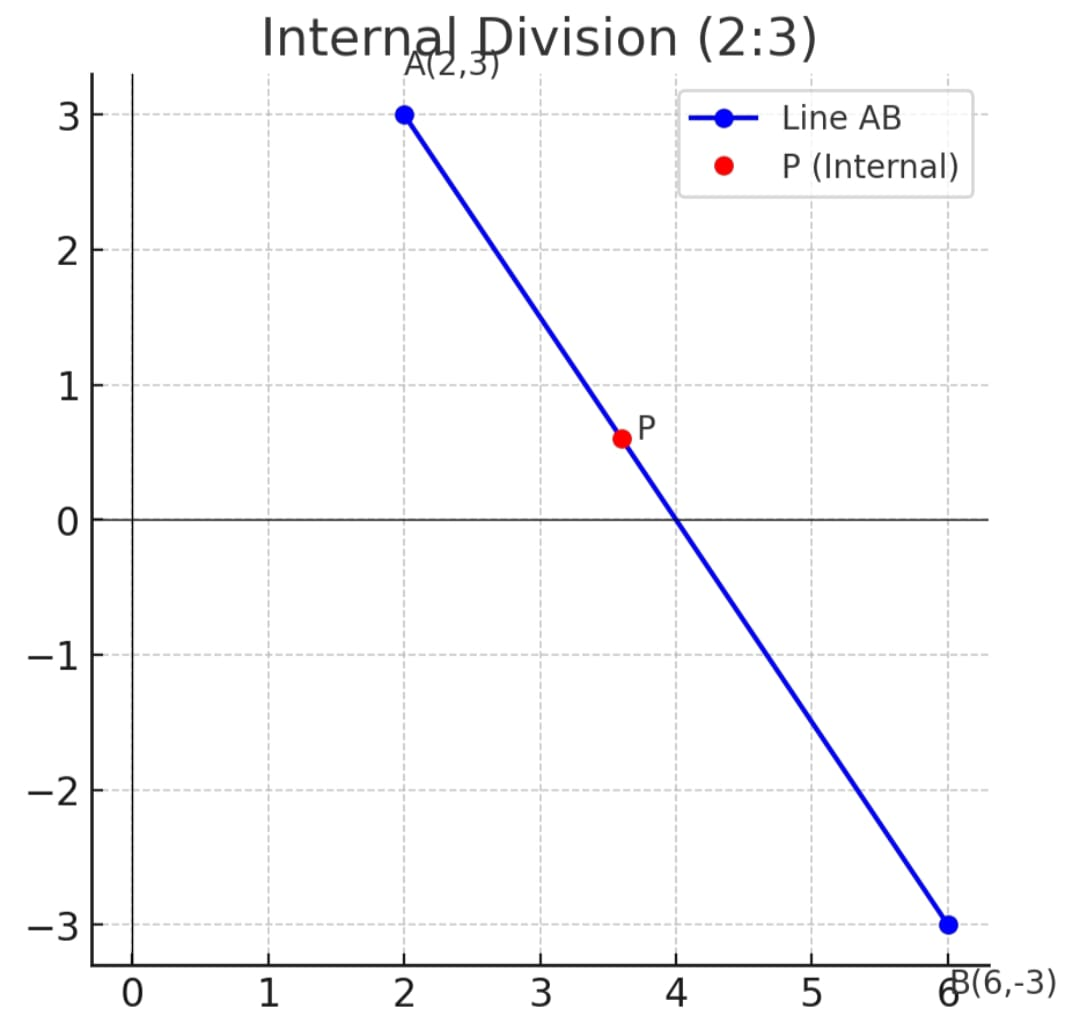
\includegraphics[width=0.55\columnwidth]{figs/fig_int_div.jpeg}
        \caption{Internal division of line AB in ratio 2:3}
    \end{figure}
\end{frame}


\begin{frame}{Plot}
    \begin{figure}
        \centering
        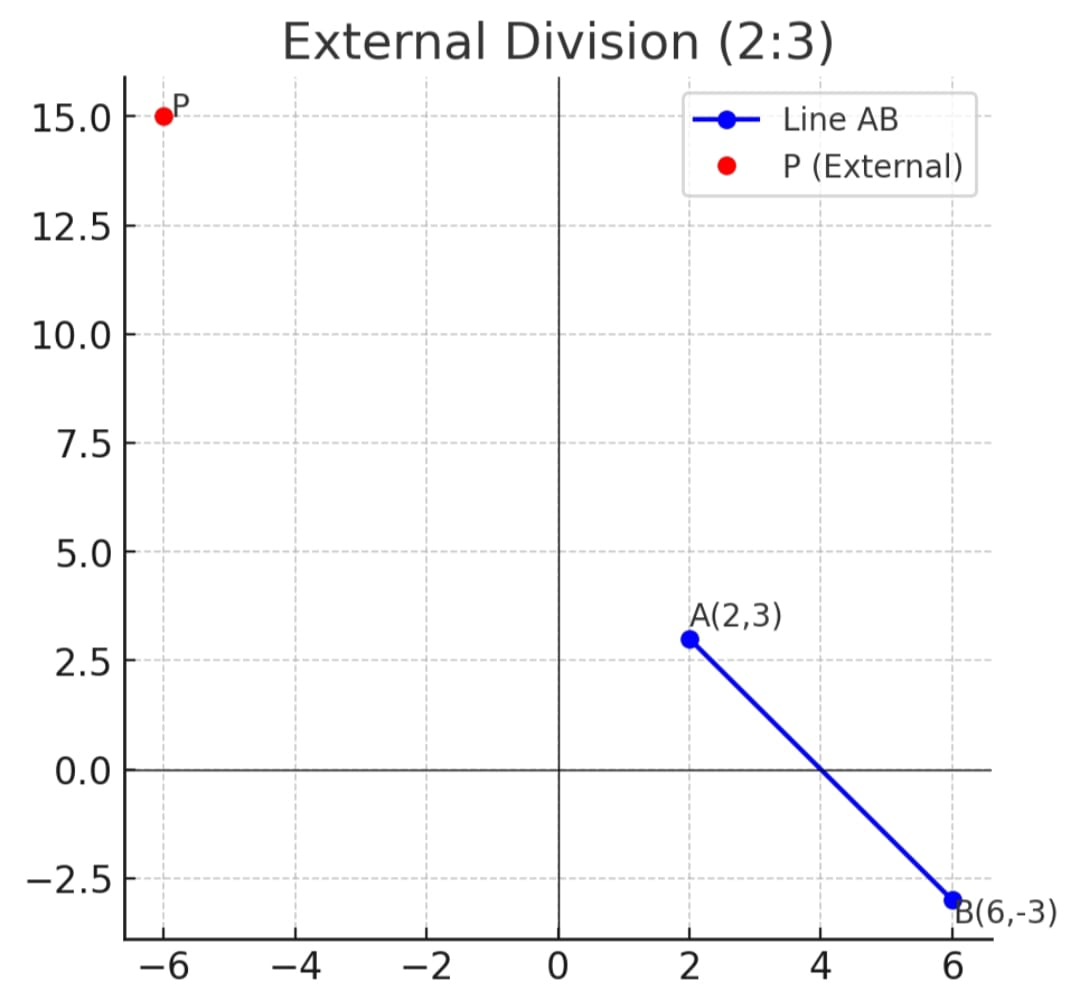
\includegraphics[width=0.55\columnwidth]{figs/fig_ext_div.jpeg}
        \caption{External division of line AB in ratio 2:3}
    \end{figure}
\end{frame}

\end{document}